\documentclass[11pt, oneside]{article}
\setlength{\parskip}{0.5em}   	% use "amsart" instead of "article" for AMSLaTeX format
\setlength\parindent{0pt}
\setlength{\abovedisplayskip}{0pt}
\setlength{\belowdisplayskip}{0pt}
\setlength{\abovedisplayshortskip}{0pt}
\setlength{\belowdisplayshortskip}{0pt}
\usepackage{geometry}                		% See geometry.pdf to learn the layout options. There are lots.
\geometry{letterpaper}                   		% ... or a4paper or a5paper or ... 
%\geometry{landscape}                		% Activate for rotated page geometry
%\usepackage[parfill]{parskip}    		% Activate to begin paragraphs with an empty line rather than an indent
\usepackage{graphicx}
\graphicspath{{images/}}				% Use pdf, png, jpg, or eps§ with pdflatex; use eps in DVI mode
\usepackage{listings}				% TeX will automatically convert eps --> pdf in pdflatex		
\usepackage{amssymb}
\usepackage{amsmath}
\usepackage[utf8]{inputenc}
\usepackage[T1]{fontenc}
\usepackage{lmodern}
\usepackage{caption}
\usepackage{floatrow}
\usepackage{color,soul}
\usepackage{ragged2e}
\usepackage{ntheorem}
\usepackage{wrapfig}
\usepackage[11pt]{moresize}
\usepackage{mwe}
\usepackage{enumitem}
\usepackage{titlesec}
\usepackage{fancyhdr}
\usepackage{needspace}


\titlespacing*{\subsection}{0pt}{0.5\baselineskip}{0.5\baselineskip}
\setlist[enumerate]{topsep=0pt}

\title{Implementation of Gibbs Sampling within Bayesian Inference and its Applications in Actuarial Science}
\author{Colton Gearhart \& Dhanuja Kasturiratna}
\date{\today}

\newcommand*{\figuretitle}[1]{
    {\centering
    \tiny{#1}
    \par\medskip}
}

\renewcommand{\footnoterule}{
  \kern -3pt
  \hrule width \textwidth
  \kern 2pt
}

\begin{document}

\title{\Large\bf Implementation of Gibbs Sampling within Bayesian Inference and its Applications in Actuarial Science}
\author{\normalsize Colton Gearhart\footnote {gearhartc1@nku.edu}\\
\normalsize Faculty advisor: Dhanuja Kasturiratna\footnote {kasturirad1@nku.edu}\\
[3pt]\normalsize Department of Mathematics and Statistics,\\
\normalsize Northern Kentucky University,\\
\normalsize Highland Heights, KY 41009, USA\\
\date{May 31, 2018}\vspace{-15pt}}%\today

\maketitle

\begin{abstract}

This paper discusses how a variety of actuarial models can be implemented and analyzed with a Bayesian approach using Gibbs sampling, a Markov chain Monte Carlo method. This approach allows a practitioner to analyze complicated actuarial models by reducing them to simpler, more manageable models. Furthermore, general properties of Gibbs sampling are discussed through a simulation approach.
\end{abstract}

\textbf{AMS 2010 subject classification:} Primary 62F40; Secondary 62E17

\textbf{Keywords and phrases:} Bayesian inference, Gibbs sampling, Markov chain, Monte Carlo simulation.

\section{Introduction}

The use of predictive models in research is a common practice for actuaries. However, they are still realizing the full potential of the many available techniques involving predictive models. The recent developments in high speed computation have opened new avenues to\vspace{10pt}\hrule \small{\textbf{Acknowledgment}: We would like to thank the Greaves Undergraduate Research Program for providing us with this opportunity and for funding our research.}

actuaries who are involved in constructing models that can be used in predicting future uncertain events. The practical development of techniques such as linear programming, dynamic programming, Monte Carlo experiments and many others would not have been possible without the arrival of high-speed computers. The actuarial profession needs to keep pace with these developments and consider how these methods can be utilized more effectively in decision making.

Stochastic models play a wide role in actuarial science applications. Mathematical analysis (a theoretical approach) is one way to extract characteristics of such models. A practitioner may also use simulation to study these models. This approach is especially useful when the stochastic models are complicated and impossible to tract theoretically. Because many actuarial models are like this, simulation is an important tool. 

This paper discusses usefulness and importance of combining Monte Carlo simulation techniques with Bayesian analysis in order to study complicated stochastic models in actuarial sciences. Bayesian analysis is quite useful as it allows one to learn about the whole distribution of a chosen quantity, rather than just a single statistic. Additionally, the assignment of probability distributions to unknown quantities allows for the reflection of uncertainty. This uncertainty is represented as the prior distribution, which is then updated with data. This increases the reliability of the estimates. Then, once suitable models for the parameters are obtained, one can study the distribution of the variables of interest, which is the end goal of Bayesian analysis.

\subsection{Bayesian Inference}\label{sec:1.1}

In classical statistical techniques, model parameters are assumed to be fixed quantities; only the data is random. Thus, probability distributions can only be used to represent the data. But in Bayesian statistics, probability distributions are often applied to more than just the data. They can represent prior uncertainty in model parameters. These then get updated with current data to produce posterior probability distributions. In effect, the parameters now contain less uncertainty; in other words, they are more informed. This thinking produces a general rule in Bayesian statistics: any quantity which has uncertainty can be represented by a probability distribution. This can be shown in Bayes' theorem, which simply is a demonstration of conditional probability, expressed using probability distributions as follows:
\[
f(\theta\mid data)=\frac{f(data\mid\theta)\,f(\theta)}{f(data)}.
\]
In this scenario, $f(\theta\mid data)$ is the posterior distribution for the parameter $\theta$. $f(data\mid\theta)$  is the sampling density for the data. This distribution is proportional to the likelihood function; however, it differs by a constant which serves to make it a proper density. $f(\theta)$ is the prior distribution for the parameter. Finally, $f(data)$ is the marginal probability of the data. When considering a continuous sample space, this marginal probability is computed as
\[
f(data)=\int{f(data\mid\theta)\,f(\theta)\,d\theta}.
\]
In words, this is the integral of the sampling density multiplied by the prior distribution over the sample space of $\theta$. This quantity is often referred to as the "marginal likelihood" for the data. It makes the posterior density proper by functioning as a normalizing constant. In addition, it is proportional to the likelihood function. These two qualities lead Bayes' theorem for probability distributions to be frequently stated as
\[
Posterior\approx Likelihood\,\times Prior.
\]
Once the posterior distribution for a parameter is derived, Bayesian analysis attempts to summarize the entire distribution. In addition to not having a reliance on asymptotic arguments about normality, this allows for numerous additional tests and summaries. Occasionally, these distributions have closed-form solutions (or at least solutions that can be computed using numerical methods). However, for many other distributions the integrals may be quite difficult or even impossible to compute, especially multivariate ones. In this instance, Monte Carlo simulation plays a major role. The general logic of sampling is to generate a sample of size $n$ from the desired distribution and then apply discrete formulas to these samples. This, in effect, approximates the integrals of interest. For example, a mean is estimated by
\[
\int xf(x)\,dx\approx\frac{1}{n}\sum x,
\]
and a variance by
\[
\int (x-\mu)^2\,f(x)\,dx\approx\frac{1}{n}\sum (x-\mu)^2.
\]
Additionally, any desired quantile can be found by noting the value of $x$ that has $Q\%$ of the sampled values below it.

To sum up, Bayesian inference commonly follows these steps:
\begin{enumerate}
\item Creating a model and obtaining posterior distributions for the parameters being studied.
\item Simulating samples from the posterior distributions.
\item Taking discrete formulas and applying them to the samples found in step 2 in order to summarize knowledge of the parameters.
\end{enumerate}

This whole process differs from the approach taken in Classical statistics, where point estimates are found for parameters and inferences are conducted using the standard error and the central limit theorem.

\subsection{Markov Chain Monte Carlo Methods and Gibbs Sampling}

One very useful class of simulation techniques is known as Markov chain Monte Carlo (MCMC) sampling methods. The purpose of using these methods is to study distributions  that would be very difficult to study otherwise (these distributions will later be referred to as "target distributions"). With the use of MCMC methods, a researcher can simulate a series of dependent random draws from models that are often quite complex. MCMC methods prove to be very useful when sampling from multivariate distributions that would normally be difficult to sample from. This is done by breaking them down into more feasible multivariate distributions or even univariate distributions.

The first step of a MCMC method is to specify a Markov chain with a unique invariant distribution equal to the target distribution (we will discuss one way to do this in the following paragraph). The next step is to generate a new value from this Markov chain given the previous value (for further reading, refer to \cite{Berg}). This forms an iterative process which produces a Markov chain of values. Furthermore, after the burn-in iterations\footnote{Burn-in iterations allow the analysis to not use the values from the first $x$ iterations where the Markov chains are attempting to converge. For our analyses, 500 iterations is considered sufficient.} are complete, it has been shown that these generated values nearly follow a random draw from the target distribution. These samples can then be used for inference procedures in a variety of ways. 

One popular MCMC method for constructing a Markov chain for a target density is Gibbs sampling. It was first introduced to the field of image restoration by Geman and Geman \cite{Geman and Geman}, however its use in the field of Bayesian analysis was first recognized by Gelfand and Smith \cite{Gelfand and Smith}. Since then, Gibbs sampling has only appeared a few times within actuarial literature. Carlin \cite{Carlin1} used Gibbs sampling to study state space modeling of non-standard actuarial time series and Carlin \cite{Carlin2} also used it to develop a Monte Carlo approach to Bayesian graduation. Klugman and Carlin \cite{Klugman and Carlin} used Gibbs sampling in a similar area, however they had a focus on Whittaker-Henderson graduation. Additionally, Scollnik \cite{Scollnik} performed a Bayesian analysis of a simultaneous equations model for insurance rate-making.

On occasion, sampling from the multivariate posterior distribution is not feasible but sampling from the conditional distributions of each parameter is possible (for further reading, refer to \cite{Besag}). In this situation, Gibbs sampling has been found to be quite applicable. To create the Markov chain, Gibbs sampling uses a set of full conditional distributions associated with the target distribution. These are then used to generate a Markov chain with a unique invariant distribution equal to the target distribution. A basic Gibbs sampling algorithm is displayed below ($j$ represents the iteration count).
\begin{enumerate}
\item[0.] Assign a vector of starting values $x^{(j)}=(x^{(j)}_1,x^{(j)}_2,\ldots,x^{(j)}_k)$, with $j=0$.
\item[1.] Set $j = j + 1$.
\item[2.] Simulate $x^{(j)}_1\sim f(x_1\mid x^{(j-1)}_2,x^{(j-1)}_3,\ldots,x^{(j-1)}_k).$
\item[3.] Simulate $x^{(j)}_2\sim f(x_2\mid x^{(j-1)}_1,x^{(j-1)}_3,\ldots,x^{(j-1)}_k).$
\item[\vdots]\hspace{1.6 cm}\vdots
\item[k.] Simulate $x^{(j)}_k\sim f(x_k\mid x^{(j-1)}_1,x^{(j-1)}_2,\ldots,x^{(j-1)}_{k-1}).$
\item[k+1.] Form $x^{(j)}=(x^{(j)}_1,x^{(j)}_2,\ldots,x^{(j)}_k).$
\item[k+2.] Return to step 1$.$
\end{enumerate}
In words, the Gibbs sampling algorithm defined above generates a random draw from each of the full conditional distributions. However, as the algorithm progresses, the values of the conditioning variables are sequentially updated. Thus, the next draw depends on the previous one. Moreover, a key aspect of Gibbs sampling is that the full conditional distribution does not need to be known; it only needs to be known up to a normalizing constant. In conjunction with a Bayesian approach, Gibbs sampling allows us to use the joint densities that have all other parameters set at their current values. In other words, with all other parameters treated as fixed, the result is often a known form of the density. This greatly reduces the difficulty of many analyses.

\section{Applications}

\subsection{Demonstrating the Properties of Gibbs Sampling} \label{Demonstrating the Properties of Gibbs Sampling}

Here we are going to study the properties of Gibbs sampling through simulation. We start by assuming the size of a claim $X$ is exponentially distributed with parameter $\lambda$. Further, we treat the parameter $\lambda$ as a random variable that follows a gamma distribution with parameters $\alpha$ and $\beta$. $\alpha$ and $\beta$ are constants. Stemming from our Bayesian approach, we can write this information as follows:
the conditional distribution of $X$ given $\lambda$ as
\begin{equation}\label{eq:1}
f(x\mid\lambda) = \lambda e^{-\lambda x},\quad\mbox{$x>0$}
\end{equation}
and the mixing distribution of $\lambda$, with parameters $\alpha$ and $\beta$ as
\[
f(\lambda\mid\alpha,\beta) = \frac{\beta^\alpha}{\Gamma(\alpha)}\lambda^{\alpha-1}e^{-\beta\lambda},\quad \mbox{$\lambda>0$}.
\]
Now, the joint distribution of $X$ and $\lambda$ can be obtained.
\begin{align*}
f(x,\lambda) &= f(x\mid\lambda)f(\lambda)\\
&= \frac{1}{\Gamma(\alpha)}\beta^\alpha\lambda^\alpha e^{-\lambda(x+\beta)}.
\end{align*}
By integrating the above joint density with respect to $\lambda$, we can obtain the marginal distribution of $X$.
\begin{align*}
f(x) &= \int_0^\infty{f(x,\lambda)\,d\lambda}\\
&= \frac{\alpha\beta^\alpha}{(\beta+x)^{\alpha+1}},\quad\mbox{$x>0$}\\
&\sim Pareto\,(\alpha,\beta).
\end{align*}
Note that $f(x)$ simplifies to a Pareto distribution with parameters $\alpha$ and $\beta$. This density is the closed form solution that was mentioned in section \ref{sec:1.1}; in most problems, this is not possible to obtain. However, we chose distributions such that there would be a closed form solution in order to compare our results to. Finally, we can solve for each conditional distribution. Having already been given $f(x\mid\lambda)$ in Equation \ref{eq:1}, $f(\lambda\mid x)$ is derived as follows:
\begin{align*}
f(\lambda\mid x) &= \frac{f(x,\lambda)}{f(x)}\\
&= \frac{(x+\beta)^{\alpha+1}\lambda^\alpha e^{-\lambda(x+\beta)}}{\Gamma(\alpha+1)}\\
&\sim gamma\,(\alpha+1,x+\beta).
\end{align*}
Notice here that the conditional distribution of $f(\lambda\mid x)$ simplifies to a gamma distribution. This is because of the use of a conjugate prior distribution. This simply means that the mixing distribution is from the same family as the variable of interest (for further reading, refer to \cite{Casella and Berger}).  

The next step in Gibbs sampling is to run our two conditional distributions through the iterative algorithm defined below:
\begin{enumerate}
\item Select arbitrary initial values $x^{(0)}$ and $\lambda^{(0)}$.
\item Set counter index $i=0$.
\item Sample $x^{(i+1)}$ from $f(x\mid\lambda^{(i)})\sim\,exponential\,(\lambda)$.
\item Sample $\lambda^{(i+1)}$ f from $f(\lambda\mid x^{(i+1)})\sim\,gamma\,(\alpha+1,x^{(i+1)}+\beta)$.
\item Set $i=i+1$ and return to step 3.
\end{enumerate}

For illustrative purposes, assume $\alpha = 5$ and $\beta = 100$. This reduces the uncertainty to the random variables $X$ and $\lambda$. Using the principles of Gibbs sampling as shown above, 100,000 random numbers are generated for $X$ and $\lambda$. Figure 1 shows the last 100 sampled values for $X$ and Figure 2 shows the last 100 sampled values for $\lambda$:

\begin{figure}[h]
   \begin{minipage}{0.45\textwidth}
      \figuretitle{Figure 1: Scatterplot of generated sample values of $X$}
      \centering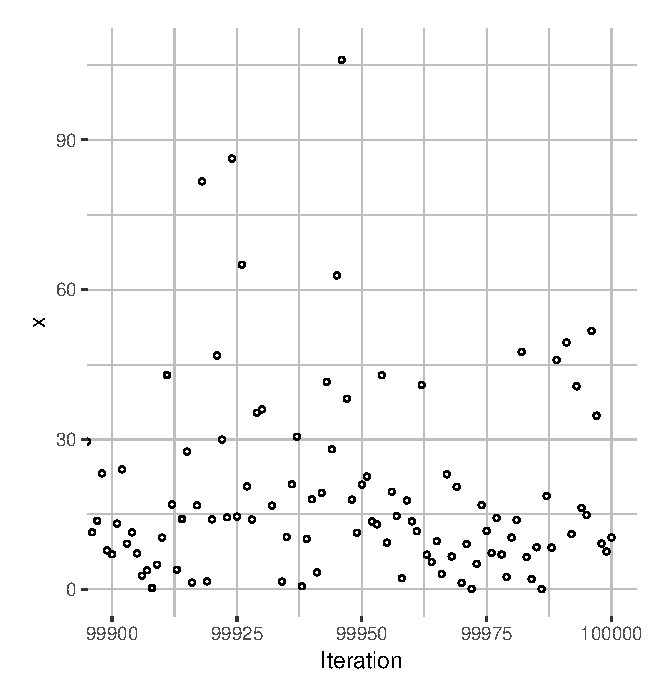
\includegraphics[scale=0.35]{Figure1}
    \end{minipage}
    \begin{minipage}{0.45\textwidth}
        \figuretitle{Figure 2: Scatterplot of generated sample values of $\lambda$}
        \centering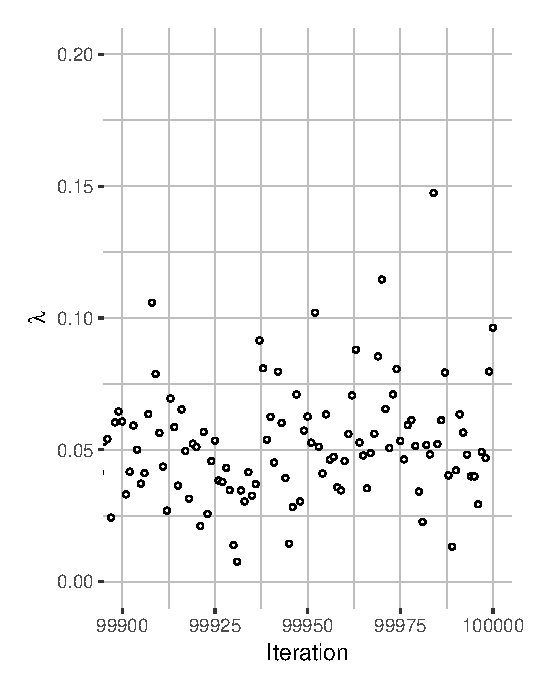
\includegraphics[scale=0.35]{Figure2}
     \end{minipage}
\end{figure}

As one can see from Figure 1 and Figure 2, there is no pattern among the generated random numbers. Therefore, they can be considered as independent random samples.

Next, Figure 3 and Figure 4 show the histograms of the last 99,500 sampled values of $X$ and $\lambda$, respectively. These values are generated from dependent sampling schemes, which were based on the full conditional distributions of $f(x\mid\lambda)$ and $f(\lambda\mid x)$. The first 500 values of each sequence are discarded as these are considered to be the burn-in iterations. Additionally, the respective marginal density curves of $X$ and $\lambda$ are overlaid on their corresponding histogram. 

\begin{figure}[h]
   \begin{minipage}{0.45\textwidth}
      \figuretitle{Figure 3: Histogram of generated sample values of $X$}
      \centering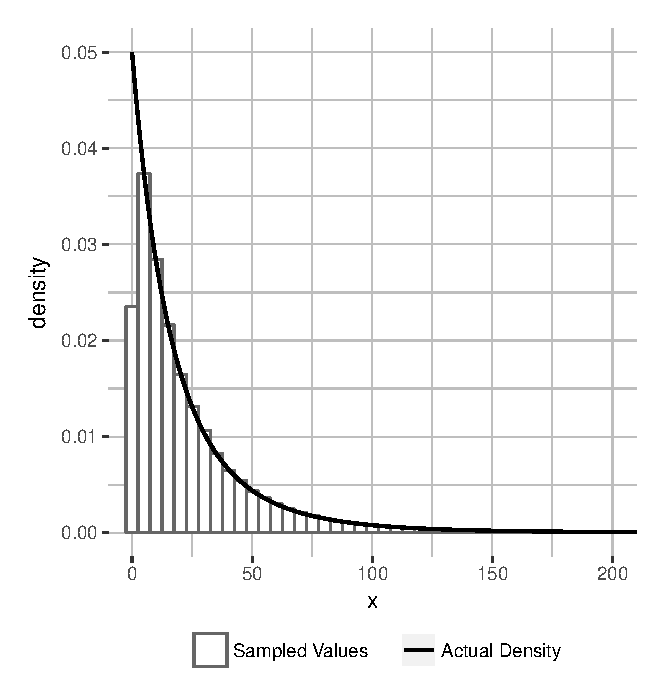
\includegraphics[scale=0.35]{Figure3}
    \end{minipage}
    \begin{minipage}{0.45\textwidth}
      \figuretitle{Figure 4: Histogram of generated sample values of $\lambda$}
        \centering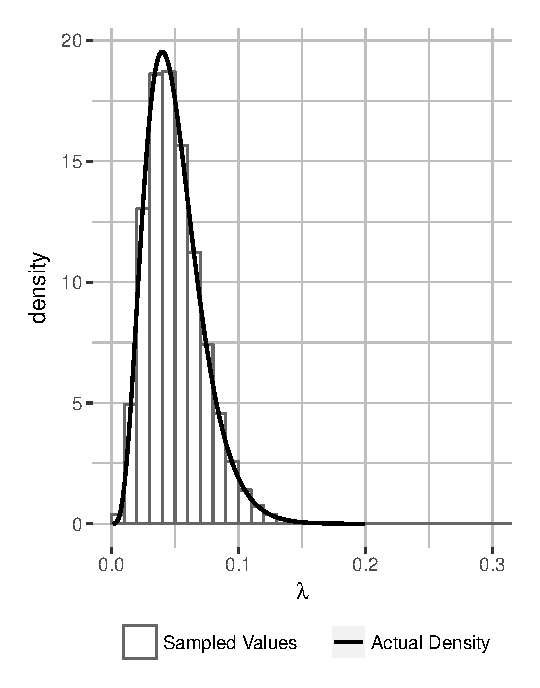
\includegraphics[scale=0.35]{Figure4}
     \end{minipage}
\end{figure}

The marginal densities appear to line up very well with the sampled values, which indicates the implemented dependent sampling schemes have generated random samples from their respective marginal distributions. 

This is a property of Gibbs sampling. In effect, by taking very large random samples from the conditional posterior distributions, it appears as if the samples were taken from their respective marginal distributions. Thus, the generated random variates can be used to study the properties of the distribution of interest. With more complicated models, sampling from the marginal distributions directly would have been impossible; but with Gibbs sampling, it can be simulated. With these results in mind, we can formally state Gibbs sampling as:

\textit{The realization that as the number of iterations approaches infinity, the samples from the conditional posterior distributions converge to what the actual target distribution is that could not be sampled from directly.}

Next, consider the following integral:
\[
f(x) = \int f(x\mid\lambda)f(\lambda)\,d\lambda.
\]
This states that the marginal distribution of $X$ can now be interpreted as the average of the conditional distribution of $X$ given $\lambda$ taken with respect to the marginal distribution of $\lambda$. This fact suggests that an estimate for the actual value of $f(x)$ at the point $x$ may be obtained by taking the simulated average of $f(x\mid\lambda)$ over the sampled values of $\lambda$, as shown in equation \ref{eq:2}. 
\begin{equation}\label{eq:2}
f(\hat{x}) = \frac{1}{99,500}\sum_{i=500}^{100,000}f(x\mid\lambda_i).
\end{equation}
A similar calculation can be done for $\lambda$.
\[
f(\hat{\lambda}) = \frac{1}{99,500}\sum_{i=500}^{100,000}f(\lambda\mid x_i).
\]
After solving for and plotting these estimated densities, direct models of their respective target distribution are revealed. The next two figures show this relationship.

\begin{figure}[h]
   \begin{minipage}{0.45\textwidth}
      \figuretitle{Figure 5: Estimated and actual density of $X$}
      \centering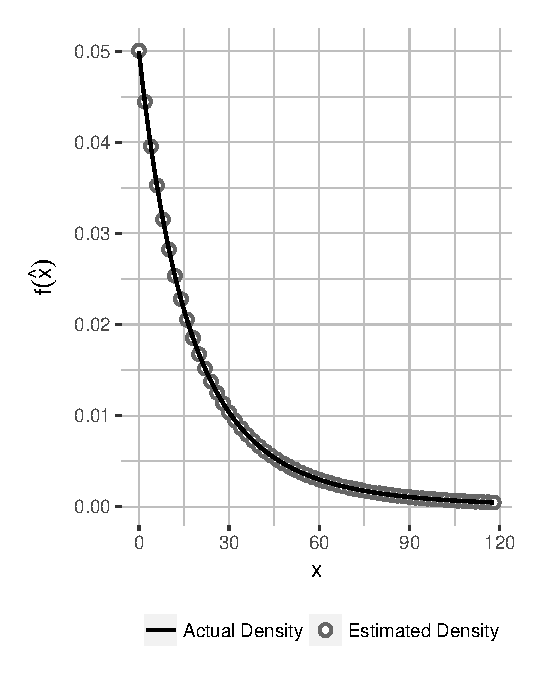
\includegraphics[scale=0.35]{Figure5}
    \end{minipage}
    \begin{minipage}{0.45\textwidth}
      \figuretitle{Figure 6: Estimated and actual density of $\lambda$}
        \centering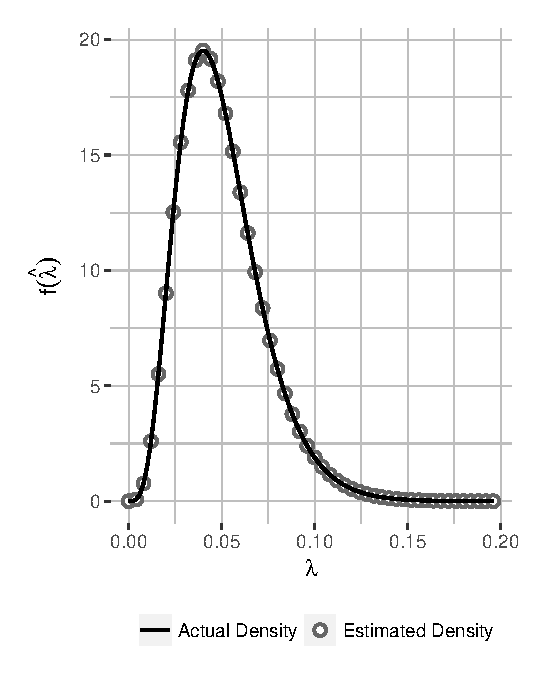
\includegraphics[scale=0.35]{Figure6}
     \end{minipage}
\end{figure}

Figure 5 shows the plotted points of $f(\hat{x})$ with its known function $f(x)$ overlaid. Figure 6 shows the same information except for $\lambda$. As one can see on both figures, the estimated densities happen to be excellent representations of the actual densities. If looking at a more complicated model where the target distribution cannot be solved for in closed form, there is now methods to solve for and study a random sample from an unknown distribution.

\subsection{Modeling Number of Claims}

\newcommand*{\permutationcombination}[4][0mu]{{{}_{#3}\mkern#1#2_{#4}}}
\newcommand*{\combination}[1][-1mu]{\permutationcombination[#1]{C}}

Actuaries often try to model the number of claims to be filed for a certain book of business. These books contain many individual policies, each with similar risk characteristics. These characteristics contribute to the probability that a claim is filed. Therefore, each book of business, which we will refer to as a portfolio, contains many policies that have a similar probability of filing a claim. This is done to allow for analyses to be completed on the group as a whole, rather than on each individual policy. 

In order to model the number of claims for a portfolio, let claim probability $P$ (as a random variable) follow a beta distribution with parameters $\alpha$ and $\beta$.
\[
f(p) = \frac{\Gamma(\alpha+\beta)}{\Gamma(\alpha)\Gamma(\beta)}p^{\alpha-1}(1-p)^{\beta-1},\quad 0\le p\le1.
\]
It is a common practice to model claim probability $P$ with a beta distribution, where the values are bounded between zero and one. In practice, distributions for probabilities of filing a claim ($P$) are skewed to the right allowing higher chances for smaller $P$'s and increasingly lower chances for higher $P$'s. The skewness of the beta distribution can easily be controlled with correctly chosen parameters $\alpha$ and $\beta$. Next, we have to model the number of policies within a certain portfolio. To do this, the Poisson distribution is widely used. However, we are going to modify it slightly. By truncating the random variable at zero (zero truncated Poisson distribution), we can ensure that the portfolio has at least one policy. Now, the total number of policies within a portfolio $N$ can be written as
\begin{align*}
f(n) &= \frac{P(N=n\mid N>0)}{1-P(N=0)}\nonumber\\
&= (e^{-\lambda}-1)\frac{\lambda^n}{n!},\quad\mbox{$n=1,2,3,\ldots$}.
\end{align*}
Next, let's focus on the number of policies that file a claim. Assuming that filing a claim for a policy is independent and that the probability of filing a claim is constant throughout the lifetime of the policy, the number of policies that file a claim $X$ can be modeled using a binomial distribution with parameters $N$ and $P$. Thus, we have
\begin{equation}\label{eq:3}
f(x\mid p,n) = \combination{n}{x}p^x(1-p)^{n-x},\quad\mbox{$x=0,1,2,\ldots,n$}.
\end{equation}
This is a well chosen distribution as it incorporates both of our previous random variates as parameters. It follows that the random variable $X$ can now be interpreted as the number of policies that generate a claim in a portfolio of $N$ identical and independent policies, each with a claim probability equal to $P$. Most often actuaries are less interested in the conditional distribution of the variable of interest, but rather the marginal distribution. This is because the marginal distribution of our random variate $X$ describes the typical number of policies generating a claim within an arbitrary portfolio; this is much more informative for them. However, $f(x)$ cannot be obtained in closed form in this particular model. Gibbs sampling is one possible solution for this problem.

As shown earlier, the first step of Gibbs sampling is to find the conditional distributions of each random variable. These are derived as follows:
\begin{align*}
f(x,p,n) &= f(x\mid p,n)f(p)f(n)\\
&= \frac{\combination{n}{x}p^{x+\alpha-1}(1-p)^{n+\beta-x-1}\Gamma(\alpha+\beta)\lambda^n}{\Gamma(\alpha)\Gamma(\beta)(e^\lambda-1)n!}
\end{align*}
\begin{align*}
f(x,n) &= \int_0^1\ f(x,p,n)\,dp\\
&= \frac{\Gamma(\alpha+\beta)\lambda^n\combination{n}{x}\Gamma(x+\alpha)\Gamma(n+\beta-x)}{\Gamma(\alpha)\Gamma(\beta)n!(e^\lambda-1)\Gamma(n+\alpha+\beta)}
\end{align*}
\begin{align}
f(p\mid x,n) &= \frac{f(x,p,n)}{f(x,n)}\nonumber\\
&= \frac{\Gamma(n+\alpha+\beta)}{\Gamma(x+\alpha)\Gamma(n+\beta-x)}p^{(x+\alpha)-1}(1-p)^{(n+\beta-x)-1}\label{eq:4}\\
&\sim beta\,(x+\alpha, n+\beta-x)\nonumber
\end{align}
\begin{align*}
f(x,p) &= \sum_{n=1}^\infty f(x,p,n)\\
&= \frac{p^{x+\alpha-1}\Gamma(\alpha+\beta)p^{\beta-1}\lambda^x(e^\lambda-1)\Gamma(\alpha)\Gamma(\beta)x!e^{\lambda(1-p)}}{\Gamma(\alpha)\Gamma(\beta)(e^\lambda-1)n!}
\end{align*}
\begin{align}
f(n\mid x,p) &= \frac{f(x,p,n)}{f(x,p)}\nonumber\\
&= \frac{e^{-\lambda(1-p)}(\lambda(1-p))^{n-x}}{(n-x)!}\quad\mbox{$n =x,x+1,x+2,\ldots$}\label{eq:5}\\
&\sim Poisson\,(\lambda(1-p)).\nonumber
\end{align}
Note that the distribution $f(p\mid x,n)$ follows a beta distribution with parameters $x+\alpha$ and $n+\beta-x$, as shown in equation \ref{eq:4}. Additionally, the conditional distribution of $N$ follows a Poisson distribution with parameter $\lambda(1-p)$, which is shown in equation \ref{eq:5}. In order to implement Gibbs sampling, we simply need to initialize the variables. For the purposes of illustration, we select $\alpha=2$ (weight on $p$) and $\beta=8$ (weight on $1-p$). This makes the distribution in equation \ref{eq:4} right skewed. Furthermore, we assume the average number of policies within a portfolio is 12 ($\lambda=12$). Next, we run a loop to generate $10,000$ random numbers from each of the full conditional distributions. We then discard the first $500$ values of each sampling path in order to burn-in Gibbs sampling. 

The output of this simulation is an approximately independent random sample from each of the conditional distributions $f(n\!\mid\! x,p)$, $f(p\!\mid\! x, n)$, and $f(x\!\mid\! p, n)$. We are interested in studying the distribution of $f(x)$, which as noted earlier could not be found in closed form. However, by averaging equation \ref{eq:3} over the simulated values $P^{(i)}$ and $N^{(i)}$, a density estimate for the random variable $X$ can be obtained. In other words, the estimated value of the density of $f(x)$ at the point $x$ is given by
\[
f(\hat{x})=\frac{1}{9,500}\sum_{i=501}^{10,000}f(x\mid p^{(i)},n^{(i)}).
\]
\begin{wrapfigure}{R}{0.3\textwidth}
   \figuretitle{Figure 7: Estimated density of $X$}
   \centering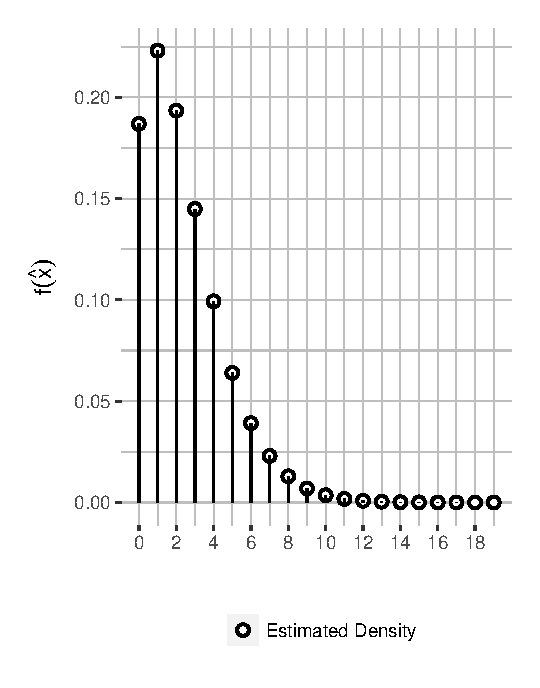
\includegraphics[width=\textwidth]{Figure7}\vspace{-30pt}
\end{wrapfigure}

A plot of this density estimate appears in Figure 7. From this, actuaries can compute many statistics for a portfolio with parameters $p$ and $n$. These can then be used to more accurately predict the number of claims expected for the future. For example, the expected value of $X$ can be found; in this case, $E(X)=0.05$ claims. Combined with a model of the size of a typical claim, this statistic can tell an insurer the amount of loss they expect per policy (in dollars). Another statistic that can be found is the variance of $X$. This tells the average risk of each portfolio. If a group of policies has a large variance, then there could potentially be a large number of claims. This implies a higher risk, which means this particular group of policies likely will have a higher premium. For this model, $Var(X)=0.0058$.

\subsection{Modeling Size of Claims}

In contrast to the previous model, which dealt with the number of claims, this one deals with the size of claims (i.e. loss amounts). Loss distributions have high probabilities for lower values and a long tail to allow for large claims, however with an increasingly smaller probability. A widely used distribution to model loss is the Pareto distribution. It incorporates parameters $\lambda$ and $\theta$ and has the following density function:
\[
f(x\mid\theta)=\frac{\theta\lambda^\theta}{(\lambda+x)^{\theta+1}},\quad\mbox{$x>0$}.
\]
Note that this distribution is a variation of the Pareto distribution called a Lomax distribution. It is essentially the same, however it has been shifted so that the support set begins at zero. To simplify the presentation, we assume that the parameter $\lambda$ is known to be 7,000 so that the only uncertainty is with respect to the value of the parameter $\theta$. Therefore, the prior distribution, represented as $\theta$, follows a gamma distribution with parameters $\alpha$ and $\beta$. In order to make further inference, again Gibbs sampling can be implemented. However, here we are considering a somewhat different situation: assume a total of 50 independent observations are available, but we only know the class frequencies (Figure 8).

\begin{center}
\figuretitle{Figure 8: Grouped data}
\begin{tabular}{|c|c|}
\hline
Class & Frequency\\
\hline
0 -- 1000&25\\
1000 -- 2000&15\\
2000 -- 3000&7\\
3000 -- $\infty$&3\\
\hline
\end{tabular}
\end{center}
If the original observations (losses) were given, the likelihood function $L(\theta\mid observations)$ can be written as
\[
L(\theta\mid observations) \propto \frac{\theta^{50}\lambda^{50\theta}}{\prod_{i=1}^{50}(\lambda+x_i)^{\theta+1}}
\]
Combining this likelihood function with the conjugate gamma $(\alpha,\beta)$ prior density for $\theta$ results in the following posterior density:
\begin{align}
f(\theta\mid observations) &\propto L(\theta)f(\theta)\nonumber\\
&\propto \frac{\theta^{50}\lambda^{50\theta}}{\prod_{i=1}^{50}(\lambda+x_i)^{\theta+1}}\frac{\beta^{\alpha}}{\Gamma(\alpha)}\theta^{\alpha-1}e^{-\beta\theta}\nonumber\\
&\propto \theta^{49+\alpha}e^{-\theta(\beta-50\ln\lambda+\sum_{i=1}^{50}\ln(\lambda+x_i))}\label{eq:6}\\
&\sim gamma\,(50+\alpha, \beta-50\ln(\lambda)+\sum_{i=1}^{50}\ln(\lambda+x_i)).\nonumber
\end{align}
Note that the conditional distribution of $\theta$ once again follows a gamma distribution, this time with parameters $50+\alpha$ and $\beta-50\ln\lambda+\sum_{i=1}^{50}\ln(\lambda+x_i)$, as shown in equation \ref{eq:6}; this is because of the conjugate nature of the gamma/Pareto distributions. Now, assume $\alpha=1$ and $\beta=0.1$. This produces a large variance in the prior distribution. These values form a vague/uninformative prior which reflects the relative ignorance of the prior distribution. While this approach is common, the practitioner should adopt whatever form of the prior density that describes the prior information actually available. Next, a procedure called data augmentation is utilized on the grouped data in order to study individual losses. The augmented data values are all independently distributed given the model parameters and each is distributed according to the Pareto density function. However, they are restricted to the appropriate class interval. Thus, the conditional distribution of the augmented data given the model parameters and the observed class frequencies is described by the following set of truncated Pareto distributions:
\begin{align}
x_i &\sim\text{truncated }Pareto\,(\theta, \lambda)\text{ on the interval (0, 1000] for $i=1,2,\ldots,25$}\label{eq:7}\\
x_i &\sim\text{truncated }Pareto\,(\theta, \lambda)\text{ on the interval (1000, 2000] for $i= 26,27,\ldots,40$}\label{eq:8}\\
x_i &\sim\text{truncated }Pareto\,(\theta, \lambda)\text{ on the interval (2000,  3000] for $i=41,42,\ldots,47$}\label{eq:9}\\
x_i &\sim\text{truncated }Pareto\,(\theta, \lambda)\text{ on the interval (3000, $\infty$) for $i=48,49,50$}\label{eq:10}.
\end{align}

\begin{wrapfigure}{R}{0.3\textwidth}
   \figuretitle{Figure 9: Sampled values of $\theta$}
   \centering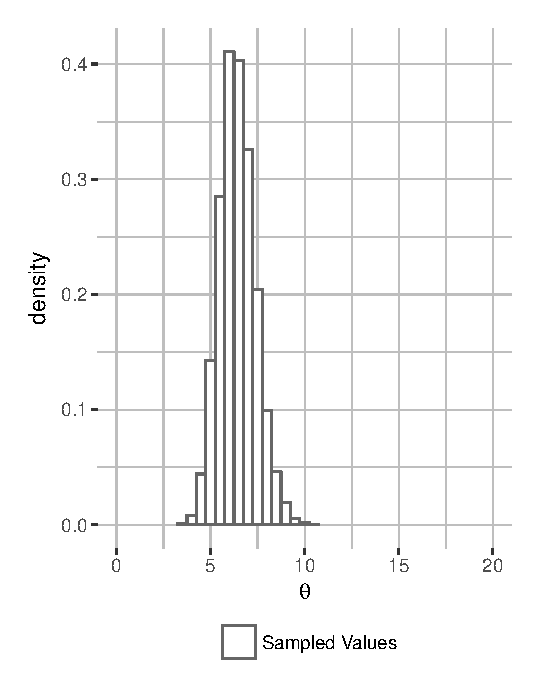
\includegraphics[width=\textwidth]{Figure9}\vspace{-50pt}
\end{wrapfigure}
By applying Gibbs sampling to the 51 full conditional distributions defined by equations \ref{eq:6} -- \ref{eq:10}, a Markov chain with an invariant distribution equal to $P(\theta,\,augmented\;data\mid observed\;data)$ can be simulated. In order to make the posterior inference with respect to $\theta$, the parameter of interest, 10,000 replications of this Markov chain are generated. Randomly selected starting values for $\theta$ and the augmented data are used each time. Additionally, let each replication run for ten iterations with only the values generated in the final iteration of each replication will be used. This technique is called thinning, which takes care of the auto-correlation effect of the generated sample. Further, by taking the last 9,500 values of the Markov chain, an approximately independent random sample from the posterior distribution $P(\theta\mid observed\;data)$ can be obtained. These values are used to construct the histogram of sample values for $\theta$ in Figure 9. The sample mean and standard deviation were 6.434 and 0.946, respectively.

By monitoring the values taken on by the augmented data as the simulation proceeds, posterior inferences can be made with respect to the actual but unobserved losses. For example, by looking at the values of the losses appearing in the upper-most class ($x_{48}$, $x_{49}$, and $x_{50}$), estimates of the posterior probability can be made that one or more of these losses exceeds an upper limit, say 10,000. Knowing a number like this can help in decision making. For this particular model, there was 1,141 observations that exceeded 10,000, giving $P(X > 10,000) \approx 3.80\%$. 

\section{Conclusions}

In this research project, we had a goal to study how the methods of Bayesian analysis combined with the insights gained from MCMC methods may be applied to areas of actuarial science. Additionally, our goal was to show how Gibbs sampling is implemented within Bayesian analysis. In practice, simulations related to Gibbs sampling are conducted through a special software WinBUGS, however our research was completed using the statistical software R \cite{R}.

There are several areas that we could have further looked into, such as how many burn-in iterations are sufficient for the conditional distributions to converge to their respective marginal distributions. This would have simply included putting a confidence band around the generated random numbers, and once they were within a previously set amount, the assumption could be made that the distributions have converged. In addition, the methods of Gibbs sampling and how the conditional distributions need to be known only up to a normalizing constant could have been further investigated. We could have also detailed more applications of the knowledge gained from Gibbs sampling. However, our methods in this paper are general and simply prove methods that can be applied to more complex problems.

\begin{thebibliography}{9}
\bibitem{Berg} Berg, Bernd A., Markov Chain Monte Carlo Simulations and Their Statistical Analysis: With Web-Based Fortran Code. Hackensack, NJ: World Scientific, 2004.\\
\bibitem{Besag} Besag, J., Spatial Interaction and the Statistical Analysis of Lattice Systems (with discussion), Journal of the Royal Statistical Society, Series B, Vol. 36, 1974, pp. 192--326.\\
\bibitem{Carlin1} Carlin, B. P., State Space Modeling of Non-Standard Actuarial Time Series, Insurance: Mathematics and Economics, Vol. 11, 1992, pp. 209--222.\\
\bibitem{Carlin2} Carlin, B. P., A Simple Monte Carlo Approach to Bayesian Graduation, Transactions of the Society of Actuaries XLIV, 1992, pp. 55--76.\\
\bibitem{Casella and Berger} Casella, G., and Berger, R.L., Statistical Inference. (2nd ed.) Pacific Grove, Calif.: Duxbury/Thomson Learning, 2002.\\
\bibitem{Gelfand and Smith} Gelfand, A. E., and A. F. M. Smith, Sampling Based Approaches to Calculating Marginal Densities, Journal of the American Statistical Association, Vol. 85, 1990, pp. 398 -- 409.\\
\bibitem{Geman and Geman} Geman, S., and D. Geman, Stochastic Relaxation, Gibbs distributions, and the Bayesian Restoration of Images, IEEE Transactions on Pattern Analysis and Machine Intelligence, Vol. 6, 1984, pp. 721 -- 741.\\
\bibitem{Klugman and Carlin} Klugman, S. A., and B. P. Carlin, Hierarchical Bayesian Whittaker Graduation, Scandinavian Actuarial Journal, Vol. 2, 1993, pp. 183--196.\\
\bibitem{R} R Core Team (2017). R: A language and environment for statistical computing. R Foundation for Statistical Computing, Vienna, Austria. URL https://www.R-project.org/.\\
\bibitem{Scollnik} Scollnik, D. P. M., A Bayesian Analysis of a Simultaneous Equations Model for Insurance Rate-Making, Insurance: Mathematics and Economics, Vol. 12, 1993, pp. 265--286.\\
\end{thebibliography}

\end{document}  